\section{FeatureSpy设计}
\label{sec:featurespy-design}

本文在设计\sysnameF 时考虑了以下设计目标:

\begin{itemize}[leftmargin=0em]
    \item \textbf{攻击检测。}\sysnameF 需可靠地检测推测内容攻击以防止客户端篡改(即具有强鲁棒性)。此外,需要实现较高的攻击检测成功率并维持较低的误判率。
    \item \textbf{保密性和带宽/存储效率。}\sysnameF 需要兼容源端重复数据删除,以达到高数据保密性和高带宽/存储效率的双重目标。此外,\sysnameF 还需减轻由于密钥泄露导致的数据块信息泄露。
    \item \textbf{低性能开销。}\sysnameF 需在上传时在线检测推测内容攻击是否发生,并在实际部署中仅产生可控且较低的性能开销。
    \item \textbf{最小化可信计算基(TCB)。}由于滥用安全区产生巨大可信计算基具有较高安全风险\cite{lie2005TCB},\sysnameF 需尽可能减小安全区大小。
\end{itemize}

本文首先提出一个安全性不足但直接的基于明文的攻击检测方案来演示本文如何通过监控数据块处理来检测推测内容攻击。然后,本文提出\sysnameF,它可以防止恶意客户端绕过推测内容攻击的检测程序。

\subsection{原型设计}
\label{subsec:featurespy-basic}

\paragraph*{概述。} 

根据推测内容攻击的执行方式,本文认为发起推测内容攻击的攻击者会枚举大量相似数据块,这些数据块均遵循相同的内容模式,并仅在有限的几个区域内发生信息变化。换句话说,这样的数据块很可能共享相同的内容特征(可以基于相应数据块的内容通过{\em N-transform}\cite{shilane12}算法生成,参见后文特征提取小节),并在一个小的时间窗口内进行处理。这导致攻击过程中每个时间窗口中数据块的内容特征分布非常偏斜。

另一方面,本文认为在实际未发生推测内容攻击的存储工作负载中,连续数据块(一起被处理的数据块)\cite{zhu2008avoiding})的特征分布通常是均匀的(即,不同的特征对应于大致相同数量的数据块)。具体来说,本文分析了两个真实世界的数据集(有关数据集的详细信息,请参阅 \S\ref{subsec:featurespy-datasets}),并将每个数据集中的数据块流划分为多个不重叠的窗口,这样每个窗口都包含$W$个连续被处理的数据块。本文通过N-transform\cite{shilane12}为每个数据块提取三个有序特征。对于每个窗口,本文计算第$i$个特征($i=1$、$2$和$3$)出现频率的标准化差值(频率的最大值与最小值的绝对差除以窗口中的总数据块个数),窗口的标准化差值越小,则表示对应的特征分布越均匀。

\begin{figure}[!htb]
    \centering
    \begin{tabular}{cc}
      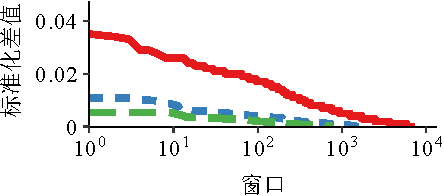
\includegraphics[width=0.45\textwidth]{pic/featurespy/plot/featureDistribution/featureDistributionLinux.pdf} &
      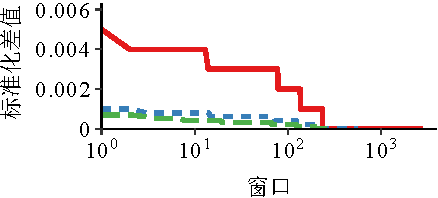
\includegraphics[width=0.45\textwidth]{pic/featurespy/plot/featureDistribution/featureDistributionCouchbase.pdf} \\
      {\small (a) Linux} & {\small (b) CouchDB} \\
      \end{tabular}
    \caption{两个真实数据集中不同窗口内数据块第一个特征频率的标准化差值(x轴上的窗口按它们的标准化差值排序)}
    \label{fig:featurespy-featureDistribution}
\end{figure}

图~\ref{fig:featurespy-featureDistribution}展示了所有窗口(大小分别为$W$=1\,K,5\,K和10\,K)基于每个数据块的第一个特征(即, $i = 1$)的标准化差异。这里,由于N-transform产生的特征具有有序性,不同顺序的特征相同的概率极低,且其他特征($i = 2$和$i = 3$)得到的结果几乎完全相同,因此本文在这里省略它们。本文观察到,尽管不同窗口之间的标准化差值分布是偏斜的,但每个窗口的标准化差值均较小。例如,在Linux数据集中仅为0.035,而在CouchDB数据集中仅为0.005。在CouchDB数据集中,当窗口大小$W$ = 1\,K、5\,K和10\,K时,分别有91.5\%、58.3\%和29.9\%的特征被相同数量的数据块共享(即特征分布均匀)。

\begin{figure}
    \centering
    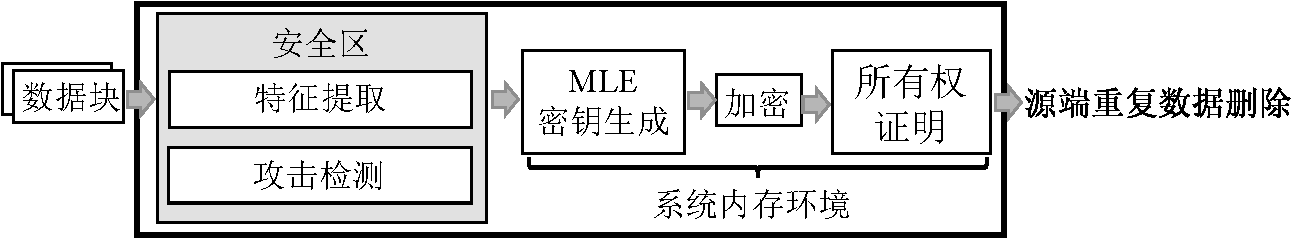
\includegraphics[width=\textwidth]{pic/featurespy/naive.pdf}
    \caption{基于明文的攻击检测方案的工作流程}
    \label{fig:featurespy-architecture-strawman}
\end{figure}

因此,基于明文的攻击检测方案通过区分特征分布来检测推测内容攻击。图~\ref{fig:featurespy-architecture-strawman}展示了基于明文的攻击检测方案的工作流程。由于攻击检测发生于客户端,为了避免攻击者修改客户端程序导致攻击检测失效,因此它通过安全区保护特征提取和攻击检测程序,从而可信地报告对推测内容攻击的检测结果。具体来说,它在安全区中提取每个明文数据块的内容特征,如果许多数据块具有相同的内容特征(即数据块相似),则报告检测到攻击。如果没有发现可疑的攻击行为,则继续执行源端加密后重复数据删除 (\S\ref{sec:background-enc-deduplication})。在下文中,本文将讨论该方案的设计细节。

\paragraph*{特征提取。}
本文通过{\em N-transform}\cite{shilane12}特征提取算法提取每个明文数据块的内容特征,该特征提取方案被广泛用于检测数据块级的相似性。N-transform是基于$N$(例如,默认为12)对系数$(a_i, m_i)$定义的,其中$N$表示有多少子特征({\em sub-features})。具体来说,对于每个明文数据块$M$,它使用Rabin指纹\cite{rabin81}对数据块上的每个32字节滑动窗口指纹,并将每个滑动窗口中的Rabin指纹$fp$转换为:

\begin{eqnarray}
  \label{eq:featurespy-feature}
  \pi_i = a_i * fp + m_i \mod 2^{32},
\end{eqnarray}

其中$i = 1, 2,\ldots, N$。如果某个Rabin指纹$fp$使得$\pi_i$为最大值,则将$M$的第$i$个子特征导出为$fp$。基本原理在于小范围的内容变化可能影响一些Rabin指纹,但其中只有少数(作为子特征)可使得$\{\pi_i\}$达到最大值。因此,对于相似的数据块,大多数子特征保持稳定。

N-transform通过将多个(例如,默认情况下为4个)连续的子特征组合在一起来计算一个特征。进而通过一组特征$S$(例如,默认情况下特征数量$|S| = 3$)来表示每个数据块,以减轻比较许多子特征以进行数据块相似性检测的计算开销。具体来说,两个数据块的共同特征越多,则它们相似的可能性越高。

\paragraph*{攻击检测。}

本文在安全区中管理一个哈希表来统计具有相同特征的明文数据块出现的频率。哈希表中的每条记录将一个特征映射到该特征在不同数据块中出现的次数(4字节)。此外,本文定义了处理窗口大小$W$(例如,默认为 5\,K)并在处理窗口中所有数据块均被处理后清空哈希表,使得哈希表中只保留当前窗口中出现的特征。这里,由于每个数据块具有三个特征,每个特征由四个子特征(4字节)连接而成,每个特征的大小为16字节,同时,每个特征使用4字节空间进行频率计数。因此,哈希表大小最大为5\,K $\times$ 3 $\times$ (16 bytes + 4 bytes) $\approx$ 300\,KiB。该哈希表在安全区中产生的内存开销可忽略不计。

为了检查每个明文数据块,本文根据其特征查询哈希表。如果某一个特征不存在,则将该特征添加到哈希表中,并将计数器置为1表示其首次出现;否则(该特征存在),本文将其对应的计数器自增1完成频率统计。如果某个特征的次数占窗口大小$W$的比率达到阈值$T$(例如,默认情况下为 3\%),本文将报告检测到推测内容攻击。

\subsection{FeatureSpy概览}
\label{subsec:featurespy-secure_design}

基于明文的攻击检测方案的一个安全缺陷是攻击检测程序容易被绕过(图~\ref{fig:featurespy-architecture-strawman-bypass})。具体来说,恶意客户端可以直接注入其自行构建的数据块执行未受保护的操作(例如,密钥生成等)处理,进而发起推测内容攻击(\S\ref{sec:background-enc-deduplication})。

\begin{figure}[!htb]
    \centering
    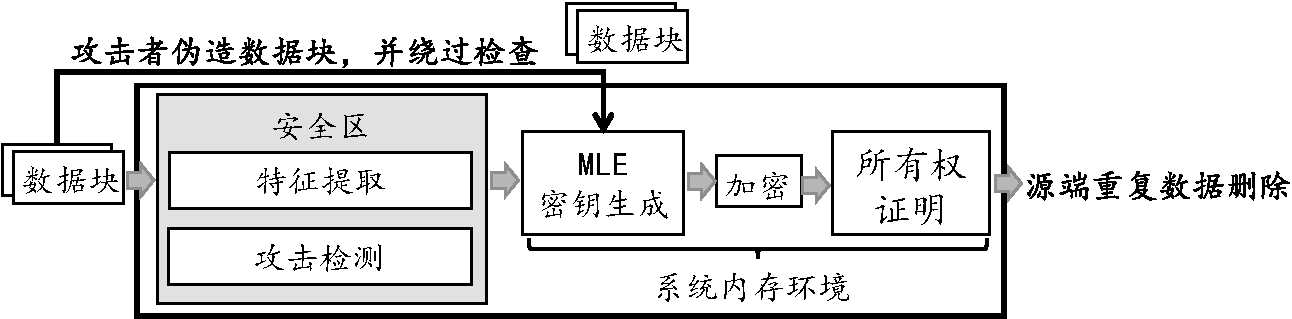
\includegraphics[width=\textwidth]{pic/featurespy/naive-problem.pdf}
    \caption{攻击检测程序被绕过}
    \label{fig:featurespy-architecture-strawman-bypass}
\end{figure}


\sysnameF 基于TEE的所有权证明方案(参见\S\ref{subsec:sgxdedup-arch})构建,以防止客户端绕过检测程序。具体来说,基于TEE的所有权证明方案将每个密文数据块作为输入并在安全区内计算密文数据块的指纹以及指纹对应的签名。进行重复数据删除时,云服务端在验证指纹对应的签名有效后才继续检查指纹是否对应于已存储的密文数据块(即发生重复数据删除)。由于云服务端仅响应具有签名的指纹,因此客户端无法对未签名的数据块进行重复数据删除查询(绕过攻击检测)。

因此,一种直接的方法是在基于明文的攻击检测方案中扩大安全区大小,以在安全区中完全推测内容攻击的检测、密钥生成、加密和基于TEE的数据所有权证明。在这种情况下,只有未修改客户端程序处理过的数据块会被云服务端接受并进行重复数据删除(由基于TEE的数据所有权证明提供保障),恶意客户端无法绕过任何程序。然而,该方法会产生巨大的可信计算基(TCB)并引入潜在的性能\cite{arnautov2016SCONE, harnik2018SGX, dinhngoc2019Everything}和安全\cite{lie2005TCB}问题。

\begin{figure}[!htb]
    \centering
    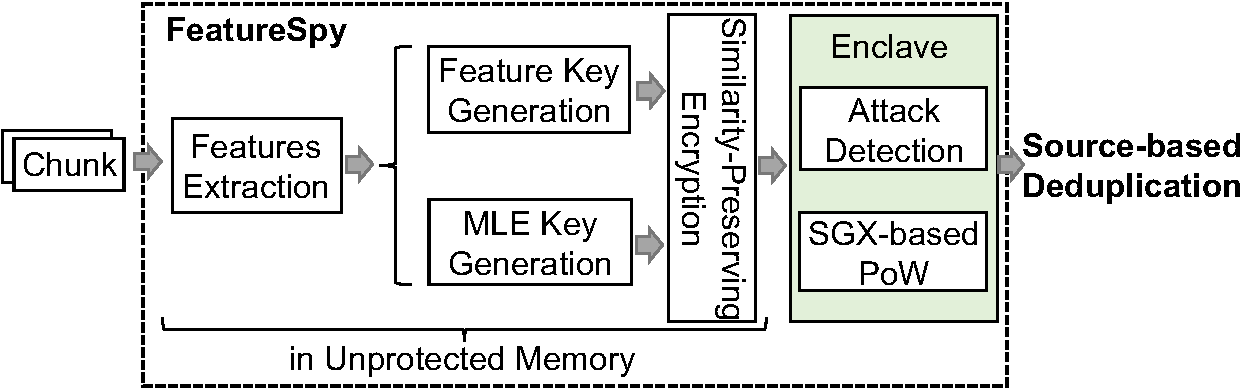
\includegraphics[width=\textwidth]{pic/featurespy/architecture.pdf}
    \caption{基于密文的攻击检测方案工作流程。\sysnameF 将攻击检测程序与安全区中的所有权证明(参见\S\ref{subsec:sgxdedup-arch})结合起来,以恶意客户端防止绕过。}
    \label{fig:featurespy-architecture-secure}
\end{figure}

\sysnameF 提出基于密文数据块的攻击检测方案,并且只将检测过程与安全区中基于TEE的数据所有权证明方案耦合(图~\ref{fig:featurespy-architecture-secure}),以减少可信计算基(TCB)的大小。

\paragraph*{挑战。}
然而,基于密文数据块的相似性检测方案提出了一个新的挑战,因为安全区只能获得加密后数据块,而在消息锁加密之后检测相似性是不可能的。因为消息锁加密密钥从明文数据块(\S\ref{sec:background-enc-deduplication})的全部内容派生加密密钥,使得相似(但不同)的数据块产生不同的加密密钥,进而导致相似的明文数据块被映射到完全不同的密文数据块,使得相似性被破坏。

本文提出一种称为基于特征的加密(Feature-based Encryption, FBE)的加密原语,它从每个明文数据块的内容特征派生加密密钥(称为特征密钥(Feature key))进行加密/解密操作。由于相似的数据块仅在少数数据区域存在不同,因此它们很可能产生相同的加密密钥。同时,相似数据块(平均大小为8\,KiB)在前几个加密块(在AES中,加密块大小为16字节)相同的概率很高。由于加密后重复数据删除\cite{douceur2002reclaiming, shah15}需要使用固定的初始化向量(IV)以保持确定性加密,且链式分组加密模式(Block-chaining encryption,例如\textit{Cipher block chaining (CBC)} 和 \textit{Cipher feedback (CFB)}\cite{dworkin01})的属性使得每个数据块在第一个不同加密块之前的所有加密块均可被加密为相同密文。基于特征的加密保持了明文相似数据块的前几个加密块高概率相同的特性,并且可以通过比较密文数据块前几个加密块是否相同判断对应的两明文数据块是否相似。

然而,基于特征的加密容易受到密钥泄露的影响,因为一个特征密钥对应于一组具有相同内容特征的数据块。恶意客户端可以使用其获得的特征密钥来完全解密多个相似数据块,特别是一些不属于攻击者本身的数据块。

这给加密后重复数据删除选择合适的加密原语带来了两难选择:消息锁加密对密钥泄露具有鲁棒性(即,泄露的消息锁加密密钥不能用于解密除相应的数据块之外的其他数据块)但会破坏相似性,而基于特征的加密保留了原始明文数据块的相似性但易受到密钥泄露的威胁。


\subsection{相似性保留加密}
\label{subsec:featurespy-spe}

本文提出了相似性保留加密(similarity-preserving
encryption, SPE),它同时建立在消息锁加密密钥和基于特征的加密之上,通过消息锁加密密钥减轻密钥泄露导致的安全威胁,同时通过基于特征的加密密文数据块相似性。具体来说(如图~\ref{fig:featurespy-design-spe}所示),由于相似数据块的内容差异有限,相似性保留加密从每个明文数据块中抽取一小部分(例如,前32个字节,占8\,KiB数据块的0.4\%),称为相似性指标({\em similarity indicator}),由此产生的相似数据块的相似性指标很可能是相同的。相似性保留加密使用基于特征的加密方案加密相似性指标,而剩余的大部分(占 8\,KiB数据块的99.6\%)数据块内容用消息锁加密。基于此,\sysnameF 可以通过检验密文数据块的相似性指标(例如,每个密文数据块的前32个字节)是否相同来检测密文数据块的相似性。由于相同的数据块共享相同的内容特征(产生相同的特征密钥)和消息锁加密密钥,消息保留加密不会降低跨用户加密后重复数据删除(\S\ref{sec:background-enc-deduplication})的存储效率。

\begin{figure}[!htb]
  \centering
  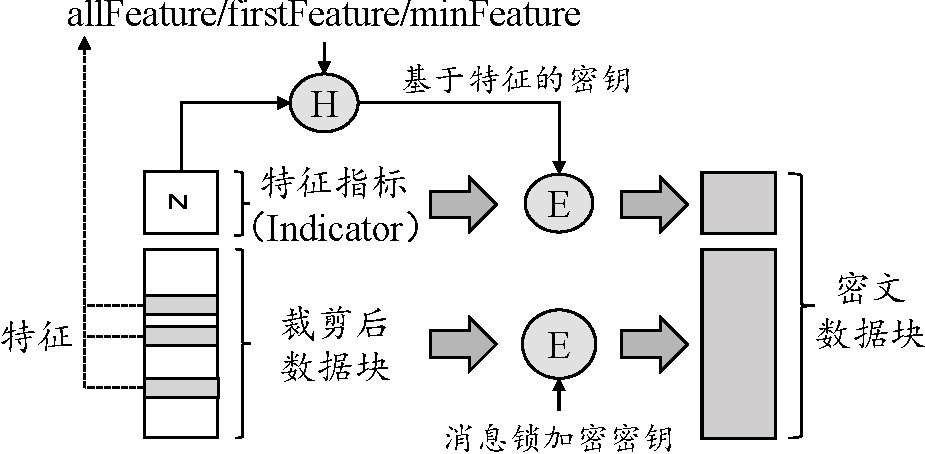
\includegraphics[width=0.7\textwidth]{pic/featurespy/spe.pdf}
  \caption{相似性保留加密方法}
  \label{fig:featurespy-design-spe}
\end{figure}

本文认为消息保留加密减轻了基于特征的加密在密钥泄露时产生的信息泄露风险。这是由于发生密钥泄露的数据块$M$对应的特征密钥只能用于解密与$M$相似的数据块的相似性指标。同时,由于相似数据块本身很可能与数据块$M$具有相同的相似性指标,因此相似性保留加密不会造成额外的信息泄露。即使是少部分与$M$相似但相似性指标不同的数据块收到该密钥泄露的影响,相较于基于特征的加密其泄露的信息也大大减少。下文将详细介绍相似性保留加密的设计细节。

\paragraph*{特征密钥生成。}
如前文所述,本文通过N-transform(\S\ref{subsec:featurespy-basic})为每个明文数据块提取三个顺序的内容特征,一个基本的密钥生成方法(称为 {\tt allFeature})是连接所有特征,并计算基于连接结果的安全哈希产生特征密钥。但是,{\tt allFeature}无法为许多相似较低的数据块生成相同的特征密钥。具体来说,如果相似数据块的内容差异恰好在产生子特征(\S\ref{subsec:featurespy-basic})的滑动窗口中,则数据块将产生不同的特征密钥,使得即使相似性指标原始内容完全相同也无法检查密文数据块的相似性。

本文基于采样的方法\cite{bhagwat2009extreme, dong2011Tradeoffs, qin17}来放宽密钥生成标准。本文为每个明文数据块的所有特征选择以一个代表特征,并根据代表特征计算特征密钥。这样可以容忍相似数据块间更大的内容差异,使得相似度较低的数据块也可产生相同的特征密钥

本文考虑了两种选择代表性特征的方法。具体来说,{\tt firstFeature}根据每个明文数据块的第一个({\em first})特征生成特征密钥。优点是不需要计算后续的子特征和特征(\S\ref{subsec:featurespy-basic}),减轻N-transform的计算开销 \cite{zhang2019Finesse}。

本文还考虑{\tt minFeature},它建立在Broder定理\cite{broder1997resemblance}的基础上,根据每个数据块所有特征中的最小({\em minimum})特征(即数值最小值)生成特征密钥。具体来说,Broder定理指出,如果两个明文数据块具有许多共同特征(即,相似的概率很高),它们很可能具有相同的最小特征,即:

\begin{eqnarray}
  \label{eq:featurespy-broder}
 \Pr[\min(S_1) = \min(S_2)] = \frac{|S_1 \cap S_2|}{|S_1 \cup S_2|},
\end{eqnarray}

其中$S_i$是明文数据块$M_i$的特征集合,$\min(S_i)$计算集合 $S_i$($i = 1, 2$)中特征的最小值。因此,{\tt minFeature}倾向于为相似度中等的数据块生成相同的特征密钥。在\S\ref{sec:featurespy-evaluation}中,本文将研究相似性保留加密的不同密钥生成方法的权衡。

此外,除了使用特征生成特征密钥外,另一种设计思路是基于第一个或最小的子特征{\em sub-feature}生成特征密钥。但由于子特征的信息熵较低,本文不选择这种基于子特征的设计。这是由于根据N-transform的原始配置\cite{shilane12},每个子特征只有4个字节,攻击者可枚举所有可能的子特征/密钥(最高 $2^{32}$)。另一方面,在\S\ref{sec:featurespy-implementation}中,本文重新配置N-transform以确保基于特征的密钥空间足够大(例如,$2^{256}$)以对抗暴力破解攻击。

\subsection{安全性分析}
\label{subsec:featurespy-security}
本文讨论了\sysnameF 的机密性保障,特别是作为底层加密原语的相似性保留加密(SPE)的安全性,并讨论了\sysnameF 应对恶意客户端的鲁棒性。

\paragraph*{对不可信云服务端的保密性。}

本文已经讨论了当密钥被泄露时相似性保留加密(SPE)相对于特征加密(FBE)的安全性提升(\S\ref{subsec:featurespy-spe}),这里关注密钥未被泄露(保持安全)时的情况。本文的目标是证明相似性保留加密(SPE)可以保护加密后重复数据删除对不可信云服务端的安全性。具体来说,由于相似性保留加密(SPE)通过消息锁加密和特征加密(FBE) 共同执行数据块加密,因此其安全性可规约为消息锁加密和特征加密的安全性。现有工作\cite{bellare2013MLE}表明,当明文数据块取自一个较大的信息空间,并且任意数据块的选取难以从信息空间中进行预测(即,明文数据块不可预测)。在下文中,本文(非正式地)说明,如果数据块特征同样不可预测,则特征加密可达到与消息锁加密同等的安全性。

本文将特征加密视为消息锁加密的一种扩展形式。如果本文将采样的特征(例如,{\tt firstFeature}和{\tt minFeature}等代指的代表特征,以及 {\tt allFeature}代指的全部特征)视为消息$M$,那么消息锁加密特征加密实际上使用$M$的安全哈希来加密对应的扩展$f(M)$(即明文数据块),其中$f(\cdot)$是一个扩展函数。由于每个$M$都是不可预测的,因此加密密钥对多项式时间的攻击者保持机密性。因此,如果底层对称加密是安全的,则攻击者无法区分产生的密文和随机值。本文的非正式分析依赖于特征不可预测的安全假设,且本文可以通过服务器辅助密钥生成\cite{bellare2013DupLESS}来增强特征密钥不可预测的假设。

\paragraph*{对恶意客户端的鲁棒性。}
本文已经讨论过攻击者无法绕过检测程序(\S\ref{subsec:featurespy-secure_design}),这里关注\sysnameF 对其他恶意行为的鲁棒性(\S\ref{sec:featurespy-setting})。

\begin{itemize}[leftmargin=*]
    \item \textbf{案例1:篡改不受保护的程序。}
    \sysnameF 通过TEE保护检测程序,但恶意客户端可以篡改未受保护的程序。它可能会操纵数据块特征、相似性指标和数据块密钥,以欺骗\sysnameF。本文认为,这些操作无助于从遵循本文设计的其他诚实客户端处获得目标内容,因为这些操作导致即使原始明文数据块是相同的,恶意客户端与相似性保留加密(由正常客户应用)产生的密文数据块不同。直接导致该密文数据块无法执行重复数据删除(被认为是非重复数据块)。最终使得依赖重复数据删除结果泄漏的推测内容攻击不可行。
    \item \textbf{案例2:篡改数据处理流程。}
    由于\sysnameF 以处理窗口为粒度检查数据块相似性,恶意客户端可能会篡改正在处理的数据块流,在正常数据块流中小心的插入相似数据块(用于攻击),使得每个窗口内只包含极少数相似数据块。尽管\sysnameF 在这种情况下无法检测到攻击,但本文认为它显著缓解了推测内容攻击。例如,在没有\sysnameF 的情况下,恶意客户端可以全部使用相似的数据块(即,数据量为$W$)填充每个窗口以发动攻击,但\sysnameF 确保攻击者在每个窗口内至多可以填充$W\times T$ 的相似块(否则会被检测到),使得攻击成本提升$1/T$倍。通过配置一个较小的阈值$T$,本文可以使推测内容攻击成本显著增高而变得不切实际。使用较小阈值的代价使增加了误判的可能性(即,将正常情况误报为检测到攻击)。
\end{itemize}
  
\paragraph*{安全性限制。}\sysnameF 基于每个独立的客户端检测推测内容攻击。但是,攻击者可能会控制多个客户端以合作发起推测内容攻击,使得每个客户端上传的相似数据块的数量大大减少,\sysnameF 可能无法有效检测到此类推测内容攻击的实施。本文将防御合作的推测内容攻击作为未来亟需解决的工作。